\section{Синтаксический анализ контекстно-свободной аппроксимации}

Наш алгоритм принимает на вход управляющие таблицы LL-анализа, построенные по эталонной грамматике, и GFG, который является представлением КС-грамматики --- аппроксимации множества значений выражения. 
Мы переиспользуем основные структуры данных и функции описанного ранее алгоритма анализа регулярной аппроксимации на основе GLL, расширяя данный подход для корректной обработки GFG.

Алгоритм последовательно обходит узлы GFG, производя синтаксический анализ порождаемых им строк. 
Для правильного построения таких строк, согласно определению выводимости строки в GFG-грамматике, для каждого просматриваемого пути необходимо поддерживать баланс call- и return-узлов. 
То есть, при прохождении пути алгоритм должен манипулировать дополнительным стеком (назовем его \textit{CR-стеком}). 
При достижении call-узла в стек добавляется номер return-узла, соответствующего ему; при достижении end-узла необходимо снять со стека номер return-узла и продолжить обход из него. 

Для экономии памяти мы не храним CR-стек для каждой из текущих ветвей работы алгоритма (напомним, что GLL-алгоритм может одновременно рассматривать несколько вариантов разбора строки). 
Вместо этого множество CR-стеков, по аналогии с основным стеком GLL-анализатора, представляется в виде GSS. 
Пример можно увидеть на рисунке \ref{fig:gss}. GSS позволяет хранить только одну копию общих префиксов нескольких стеков, каждый путь в нем соответствует отдельному CR-стеку.

\begin{figure}[h]
	\centering
	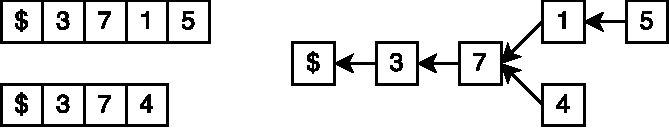
\includegraphics[width=6cm]{pictures/kovalev-spbu-gss_cr}
	\caption{Структурированный в виде графа стек}
	\label{fig:gss}
\end{figure}

Для хранения указателя на текущую вершину стека мы добавили в дескрипторы дополнительное поле. 
Таким образом, дескриптором в нашем алгоритме называется пятерка вида $(L, u, i, N, s)$, где $i$ --- номер вершины GFG, $s$ --- указатель на вершину CR-стека в GSS, остальные поля аналогичны тем, которые представлены в дескрипторах оригинального GLL-алгоритма.

Другой особенностью работы с GFG является то, что он, в отличие от регулярной аппроксимации --- детерминированного конечного автомата, допускает возможность неоднозначного выбора пути обхода. 
Подобная ситуация возникает при наличии в исходной грамматике нескольких продукций, содержащих в левой части одинаковый нетерминал. 
Например, GFG на рисунке \ref{fig:gfg} содержит start-узел под номером 3, из которого выходит два ребра с пустой меткой (аналог $\epsilon$-переходов в конечном автомате).

Механизм дескрипторов позволяет решать проблему недетерминированного выбора пути --- для каждого из возможных вариантов создается отдельный дескриптор, который добавляется в очередь исполнения. 
Вернемся к примеру с узлом 3 на рисунке \ref{fig:gfg}. Пусть в текущий момент времени мы имеем дескриптор $(L_1, u_1, i_1, N_1, s_1)$. 
При рассмотрении ребер, выходящих из узла 3, будут созданы дескрипторы $(L_1, u_1, 4, N_1, s_1)$ и $(L_1, u_1, 5, N_1, s_1)$. Если ранее такие дескрипторы не создавались (для контроля за этим в GLL поддерживается глобальное множество создаваемых дескрипторов), они будут добавлены в очередь.

Функции \textbf{dispatcher} и \textbf{add} (проверка и добавление в очередь дескриптора) алгоритма анализа регулярной аппроксимации были незначительно изменены нами для работы с расширенными дескрипторами. 
Функция \textbf{processing} и методы для работы с основным стеком и построения SPPF переиспользованы без изменений.
Обработка start/call/exit-узлов и контроль за состоянием CR-стеков были реализованы во вспомогательной функции \textbf{closure}, псевдокод которой приведен ниже.
Она исполняется перед вызовами \textbf{dispatcher} и \textbf{processing}, производя рекурсивный обход GFG до тех пор, пока не встретит start- или scan-узел. 
При достижении start-узла создаются дескрипторы для каждого из возможных путей, и управление переходит к \textbf{dispatcher};
scan-узел обрабатывается функцией \textbf{processing} так же, как и вершина конечного автомата в оригинальном алгоритме.

\begin{algorithmic}
	
\Procedure{closure}{}
	\State tuple $(C_L, C_u, C_i, C_N, C_S)$ is the current state of the analysis process
	\State $v \gets$ current GFG vertex
	\If{($v$ is not a final vertex)}
		\Switch{$VertexType(v)$}
			\Case{$Start$}
				\For{$(e \in v.OutputEdges)$}
					\State \Call{add}{$e.Target, C_L, C_u, C_N, C_S$}
				\EndFor
			\EndCase
			\Case{$Call(r)$ where $r$ is matching return vertex}
				\State add CR-stack vertex $w$ labeled $r$ and edge from $w$ to $C_S$
				\State $C_S \gets w$
				\State $C_I \gets$ target vertex of $v.OutputEdge$
				\State \Call{closure}{}
			\EndCase
			\Case{$Exit$}
				\State let $w$ be the target vertex of $v.OutputEdge$
				\If{($w$ is not a final vertex)}
					\State $C_I \gets C_S.Label$
					\State $C_S \gets$ predecessor of $C_S$ in CR-stack
					\State \Call{closure}{}
				\Else
					\State $C_I \gets w$
				\EndIf
			\EndCase
			\Case{\_}
				\ \Return
			\EndCase
		\EndSwitch
	\EndIf
\EndProcedure
\end{algorithmic}

Результатом работы алгоритма является SPPF, представляющий набор деревьев разбора строк, порождаемых GFG и одновременно с этим выводимых в эталонной грамматике.
Отметим, что SPPF может быть построен не всегда, так как класс КС-языков не замкнут относительно пересечения.